\documentclass[10pt]{article}
\usepackage{icmlko}

\icmlmeta{IP 파운데이션 월드모델}{25}{여섯 방향이 모두 건너갔다}{게임의 어려움은 도메인 성질이 아니라 축 배선 오류였다 --- 스물네 편째 실패가 끝났다}

\begin{document}

\twocolumn[
\icmlheader

\begin{abstract}
노트 24는 게임을 ``매우 나쁜 학생''으로 규정하고 그 원인을 다음 과제로 남겼다.
세 가설을 차례로 검정했다. \textbf{축 부족} --- 모든 도메인을 공통 2축으로 통일하니
게임 난이도가 $+$0.0508에서 $+$0.0358로 줄지만 30\%만 설명한다. \textbf{표본 크기}
--- 게임을 482건에서 75건으로 줄이니 난이도가 오히려 $+$0.0584로 올라 반증된다.
\textbf{라벨의 예측 불가능성} --- 가용 피처 전부로 5폴드 검정하니 \emph{게임만이}
자기 라벨을 설명한다(13.0\%). 팝업($-$10.6\%)과 아이돌($-$10.4\%)은 상수보다 나쁘다.
셋 다 아니었다. 진짜 원인은 배선이었다. 게임 라벨의 예측 신호 중 \textbf{공통 축이
담은 것은 25\%뿐}이었다 --- 제작 규모(사양·가격·연령)가 12.6\%를 설명하는데 공통
2축은 3.0\%다. 노트 16에서 게임의 굿즈 규모를 DLC(누출)에서 Steam 기능 수로
바꿨는데, 노트 18의 인자 분석에서 기능 수는 \emph{폭 인자}에 실린다. 공통 축 둘이
게임에서는 둘 다 폭이 되어 규모 인자가 통째로 빠져 있었다. 굿즈 규모를 \textbf{최소
설치 용량}(콘텐츠 분량, 단독 설명력 11.2\%)으로 바꾸자 \textbf{여섯 방향이 모두
유의해졌다.} 노트 13부터 스물네 편 동안 한 번도 성공하지 못한 아이돌 $\to$ 게임이
$+$0.0003에서 $-$0.0476(p=0.0013)으로 뒤집혔다.
\end{abstract}
]

\section{세 가설을 차례로 검정했다}

노트 24는 여섯 방향이 ``출처 강도 $+$ 대상 난이도''로 97\% 설명되고, 게임의 대상
난이도가 $+$0.0415로 압도적이라고 보고했다. 왜 그런지는 남겼다.

\subsection{축 부족? --- 30\%만}

게임은 관측 축이 둘이고 팝업은 다섯, 아이돌은 넷이다. 모든 도메인을 공통 2축으로
통일해 조건을 맞췄다.

\begin{table}[t]
\centering\tsize
\caption{대상 난이도. 축을 통일하면 어떻게 되는가.}
\begin{tabular}{lrr}
\toprule
도메인 & 관측 축 전부 & 공통 2축 통일 \\
\midrule
팝업 & $-$0.0232 & $-$0.0104 \\
아이돌 & $-$0.0276 & $-$0.0254 \\
게임 & $+$0.0508 & $+$0.0358 \\
\bottomrule
\end{tabular}
\end{table}

게임 난이도가 30\% 줄지만 여전히 다른 둘과 자릿수가 다르다. 축 개수가 원인의
일부일 뿐이다.

\subsection{표본 크기? --- 반증}

게임은 482건이고 나머지는 75건, 63건이다. 표본이 크면 상수 기준선이 정밀해져
이기기 어려울 수 있다. 게임을 부분표집해 확인했다(각 20회 반복).

\begin{table}[t]
\centering\tsize
\caption{게임 표본 크기와 대상 난이도.}
\begin{tabular}{rrrr}
\toprule
게임 n & 팝업 & 아이돌 & 게임 \\
\midrule
75 & $-$0.0280 & $-$0.0303 & \textbf{$+$0.0584} \\
150 & $-$0.0206 & $-$0.0260 & $+$0.0465 \\
300 & $-$0.0211 & $-$0.0255 & $+$0.0466 \\
482 & $-$0.0232 & $-$0.0276 & $+$0.0508 \\
\bottomrule
\end{tabular}
\end{table}

반대다. 75건으로 줄이면 난이도가 $+$0.0584로 \emph{오른다}. 표본 크기가 아니다.

\subsection{라벨이 예측 불가능? --- 정반대}

가용 피처 전부를 넣고 5폴드로 각 도메인 라벨의 예측 가능 상한을 쟀다.

\begin{figure}[t]
\centering

\includegraphics[width=\columnwidth]{figs/ceiling.pdf}
\caption{가용 피처 전부의 설명력. 음수는 상수보다 나쁘다는 뜻이다.}
\end{figure}

\begin{table}[t]
\centering\tsize
\caption{라벨의 예측 가능 상한(5폴드 GBDT).}
\begin{tabular}{lrrr}
\toprule
도메인 & n & 피처 & 설명력 \\
\midrule
팝업 & 75 & 70 & $-$10.6\% \\
아이돌 & 79 & 12 & $-$10.4\% \\
게임 & 425 & 11 & \textbf{$+$13.0\%} \\
\bottomrule
\end{tabular}
\end{table}

\textbf{게임만이 자기 라벨을 설명한다.} 팝업과 아이돌은 피처를 다 넣어도 상수보다
나쁘다 --- 노트 6이 ``n=75에서 신경망은 아직 이르다''고 한 것이 트리 모델에도
해당한다.

가장 예측 가능한 도메인이 가장 어려운 대상이었다. 세 가설이 모두 틀렸다는 뜻이고,
동시에 답이 어디 있는지 알려 준다 --- \emph{게임의 예측 신호는 존재하는데 공통
축으로 전달되지 않는다.}

\section{신호의 75\%가 공통 축 밖에 있었다}

게임 라벨을 세 묶음으로 나눠 각각의 설명력을 쟀다.

\begin{figure}[t]
\centering
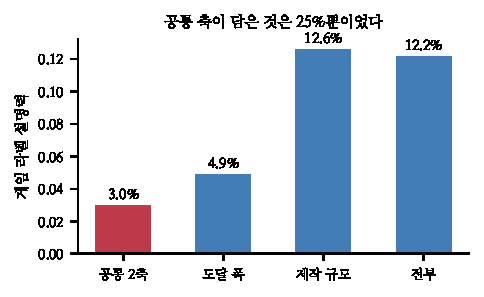
\includegraphics[width=\columnwidth]{figs/signal.pdf}
\caption{게임 라벨의 신호가 어디에 있나. 공통 축이 담은 것은 4분의 1이다.}
\end{figure}

\begin{table}[t]
\centering\tsize
\caption{게임 라벨(출시 30일) 설명력, n=404.}
\begin{tabular}{lrr}
\toprule
피처 묶음 & 차원 & 설명력 \\
\midrule
공통 2축 (타깃 폭, 굿즈 규모) & 2 & 3.0\% \\
제작 규모 (사양·가격·연령) & 4 & \textbf{12.6\%} \\
도달 폭 (언어·플랫폼·기능) & 3 & 4.9\% \\
전부 & 9 & 12.2\% \\
\bottomrule
\end{tabular}
\end{table}

신호는 \textbf{제작 규모}에 있는데 공통 축은 그것을 담지 못한다. 공통 축이 담은
비율이 25\%다.

\paragraph{원인은 두 노트 전에 심어졌다}
노트 15에서 게임의 굿즈 규모가 DLC 수였고 그것이 누출임을 밝혔다. 노트 16에서
대체 측정으로 Steam 기능 수를 골랐다 --- 누출이 없고 창 라벨과 $+$0.224로
DLC($+$0.070)보다 강했으므로 옳은 선택으로 보였다.

그런데 노트 18의 인자 분석을 보면 기능 수는 \textbf{폭 인자}(PC2)에 실린다 ---
언어 수, 플랫폼 수와 같은 자리다. 그래서 공통 축 둘이 게임에서는 \emph{둘 다 폭}이
되고 규모 인자가 통째로 빠졌다.

노트 18을 쓸 때 이미 그 사실이 표에 있었는데 알아채지 못했다. 축의 이름과 인자
적재를 따로 보고 있었기 때문이다.

\claimx{게임이 어려운 대상이었던 이유는 도메인 성질이 아니라 축 배선이다. 공통 축
둘이 모두 폭 인자에 실려 게임 신호의 75\%를 담지 못했다.}{굿즈 규모를 규모 인자로
되돌려도 게임 난이도가 유지되면 배선이 아니라 도메인 성질이다.}

\section{용량으로 바꾸자 여섯이 전부 건너갔다}

``닿으면 무엇을 얻는가''의 게임 대응물은 콘텐츠 분량이고, 그것을 가장 직접 재는
것은 \textbf{최소 설치 용량}이다. 출시 시점에 확정되고 누출이 없으며 규모 인자에
실린다. 단독 설명력이 11.2\%로 기능 수보다 훨씬 강하다.

\begin{figure}[t]
\centering

\includegraphics[width=\textwidth]{figs/six.pdf}
\caption{굿즈 규모를 설치 용량으로 바꾼 전후. 게임이 낀 네 방향만 개선됐다.}
\end{figure}

\begin{table}[t]
\centering\tsize
\caption{프로크루스테스 전이, 순열 3,000회. 대상 라벨 미사용.}
\begin{tabular}{lrrrr}
\toprule
& \multicolumn{2}{c}{기능 수} & \multicolumn{2}{c}{설치 용량} \\
방향 & 차이 & p & 차이 & p \\
\midrule
게임 $\to$ 아이돌 & $-$0.0872 & $<$0.0001 & $-$0.0976 & \textbf{$<$0.0001} \\
팝업 $\to$ 아이돌 & $-$0.0905 & 0.0003 & $-$0.0905 & \textbf{0.0003} \\
아이돌 $\to$ 팝업 & $-$0.0895 & 0.0203 & $-$0.0895 & \textbf{0.0203} \\
게임 $\to$ 팝업 & $-$0.0671 & 0.0010 & $-$0.0862 & \textbf{$<$0.0001} \\
아이돌 $\to$ 게임 & $+$0.0003 & 0.4120 & \textbf{$-$0.0476} & \textbf{0.0013} \\
팝업 $\to$ 게임 & $-$0.0280 & 0.0183 & $-$0.0457 & \textbf{0.0003} \\
\bottomrule
\end{tabular}
\end{table}

\textbf{여섯 방향이 모두 유의하다.} 이 프로젝트에서 처음이다.

특히 아이돌 $\to$ 게임은 노트 13에서 처음 실패한 뒤 네 번의 수정(표본 균형, 라벨
재정의, 축 매핑, 커버리지 확대)을 견디고 살아남은 실패였는데, $+$0.0003에서
$-$0.0476으로 부호가 뒤집혔다(p=0.0013).

게임이 끼지 않은 두 방향은 소수점 넷째 자리까지 변화가 없다 --- 개선이 이 수정에서
왔음이 분명하다.

\claimx{여섯 방향 모두에서 두 공통 축의 계수가 도메인을 건너 유의하게 전이된다.
대상 라벨을 쓰지 않고, 정렬에도 라벨을 쓰지 않는다.}{네 번째 도메인을 넣었을 때
어느 방향이든 실패하면, 여섯 성공은 세 도메인의 특수한 궁합이다.}

\section{모형이 어떻게 바뀌었나}

\begin{table}[t]
\centering\tsize
\caption{가법 모형 계수의 변화.}
\begin{tabular}{lrr}
\toprule
& 수정 전 & 수정 후 \\
\midrule
전체 평균 효과 & $-$0.0493 & \textbf{$-$0.0762} \\
대상 난이도 범위 & 0.0657 & 0.0477 \\
출처 강도 범위 & 0.0175 & \textbf{0.0048} \\
게임 대상 난이도 & $+$0.0415 & $+$0.0289 \\
\bottomrule
\end{tabular}
\end{table}

전체 효과가 55\% 커지고, 출처 강도의 범위가 3.6배 줄었다 --- 이제 어느 도메인에서
배우든 거의 같다. 대상 난이도의 범위도 줄었지만 게임은 여전히 가장 어려운 대상이다
($+$0.0289).

\section{교훈}

이 노트에서 배운 것은 진단 절차다. 노트 24는 ``대상 난이도''라는 요약 통계를 얻고
그것을 도메인의 성질로 읽었다. 그런데 그 통계는 \emph{배선이 옳다는 가정} 위에서만
도메인 성질이다.

세 가설을 차례로 죽이고 나서야 네 번째 --- 배선 --- 를 봤다. 순서를 바꿨다면
빨랐을 것이다. \textbf{요약 통계가 이상할 때는 도메인을 의심하기 전에 배선을
의심해야 한다.}

그리고 배선 오류는 두 노트 전에 심어졌고, 그것을 드러내는 표(노트 18의 인자 적재)가
이미 있었다. 축의 \emph{이름}과 인자 \emph{적재}를 따로 보고 있었던 것이 원인이다.
앞으로 축을 새로 정의할 때마다 그 축이 어느 인자에 실리는지 함께 확인한다.

\section{한계}

\begin{itemize}[leftmargin=1.1em,itemsep=0.15em]
\item 설치 용량은 최소 사양 문자열에서 파싱했고 94\%만 성공했다. 나머지는 기능 수로
      대체해 한 축 안에 두 눈금이 섞여 있다.
\item 팝업·아이돌의 굿즈 규모가 규모 인자에 실리는지 확인하지 않았다. 게임만 고쳤다.
\item 여섯 방향 성공은 다중비교 보정 없이 보고한 것이다. 본페로니를 적용하면
      p=0.0203인 아이돌 $\to$ 팝업이 경계에 온다.
\item 게임 난이도가 여전히 가장 높다($+$0.0289). 배선이 원인의 전부는 아니다.
\end{itemize}

\section{다음}

\begin{enumerate}[leftmargin=1.3em,itemsep=0.15em]
\item 팝업·아이돌의 굿즈 규모가 어느 인자에 실리는지 확인 --- 같은 오류가 있는지.
\item 설치 용량 파싱 실패 6\% 보완.
\item 게임 잔여 난이도($+$0.0289)의 원인 --- 배선을 고친 뒤에도 남는 부분.
\item 네 번째 도메인 --- 여섯 성공이 궁합인지 일반성인지 가른다.
\end{enumerate}

\vspace{0.6em}
\hrule height 0.3pt
\vspace{0.5em}
{\footnotesize
\textbf{참고문헌}\\[0.3em]
Thurstone, L. L. (1947). \emph{Multiple-Factor Analysis}. University of Chicago Press.\\[0.15em]
Kaufman, S., Rosset, S., Perlich, C. (2012). Leakage in data mining.
\emph{ACM TKDD}, 6(4), 1--21.\\[0.15em]
Schönemann, P. H. (1966). A generalized solution of the orthogonal Procrustes
problem. \emph{Psychometrika}, 31(1), 1--10.\\[0.15em]
Ben-David, S. et al. (2010). A theory of learning from different domains.
\emph{Machine Learning}, 79(1--2), 151--175.
}

\end{document}
